% Options for packages loaded elsewhere
\PassOptionsToPackage{unicode}{hyperref}
\PassOptionsToPackage{hyphens}{url}
\PassOptionsToPackage{dvipsnames,svgnames,x11names}{xcolor}
%
\documentclass[
  letterpaper,
  DIV=11,
  numbers=noendperiod]{scrartcl}

\usepackage{amsmath,amssymb}
\usepackage{iftex}
\ifPDFTeX
  \usepackage[T1]{fontenc}
  \usepackage[utf8]{inputenc}
  \usepackage{textcomp} % provide euro and other symbols
\else % if luatex or xetex
  \usepackage{unicode-math}
  \defaultfontfeatures{Scale=MatchLowercase}
  \defaultfontfeatures[\rmfamily]{Ligatures=TeX,Scale=1}
\fi
\usepackage{lmodern}
\ifPDFTeX\else  
    % xetex/luatex font selection
\fi
% Use upquote if available, for straight quotes in verbatim environments
\IfFileExists{upquote.sty}{\usepackage{upquote}}{}
\IfFileExists{microtype.sty}{% use microtype if available
  \usepackage[]{microtype}
  \UseMicrotypeSet[protrusion]{basicmath} % disable protrusion for tt fonts
}{}
\makeatletter
\@ifundefined{KOMAClassName}{% if non-KOMA class
  \IfFileExists{parskip.sty}{%
    \usepackage{parskip}
  }{% else
    \setlength{\parindent}{0pt}
    \setlength{\parskip}{6pt plus 2pt minus 1pt}}
}{% if KOMA class
  \KOMAoptions{parskip=half}}
\makeatother
\usepackage{xcolor}
\setlength{\emergencystretch}{3em} % prevent overfull lines
\setcounter{secnumdepth}{-\maxdimen} % remove section numbering
% Make \paragraph and \subparagraph free-standing
\makeatletter
\ifx\paragraph\undefined\else
  \let\oldparagraph\paragraph
  \renewcommand{\paragraph}{
    \@ifstar
      \xxxParagraphStar
      \xxxParagraphNoStar
  }
  \newcommand{\xxxParagraphStar}[1]{\oldparagraph*{#1}\mbox{}}
  \newcommand{\xxxParagraphNoStar}[1]{\oldparagraph{#1}\mbox{}}
\fi
\ifx\subparagraph\undefined\else
  \let\oldsubparagraph\subparagraph
  \renewcommand{\subparagraph}{
    \@ifstar
      \xxxSubParagraphStar
      \xxxSubParagraphNoStar
  }
  \newcommand{\xxxSubParagraphStar}[1]{\oldsubparagraph*{#1}\mbox{}}
  \newcommand{\xxxSubParagraphNoStar}[1]{\oldsubparagraph{#1}\mbox{}}
\fi
\makeatother

\usepackage{color}
\usepackage{fancyvrb}
\newcommand{\VerbBar}{|}
\newcommand{\VERB}{\Verb[commandchars=\\\{\}]}
\DefineVerbatimEnvironment{Highlighting}{Verbatim}{commandchars=\\\{\}}
% Add ',fontsize=\small' for more characters per line
\usepackage{framed}
\definecolor{shadecolor}{RGB}{36,41,46}
\newenvironment{Shaded}{\begin{snugshade}}{\end{snugshade}}
\newcommand{\AlertTok}[1]{\textcolor[rgb]{1.00,0.33,0.33}{\textbf{#1}}}
\newcommand{\AnnotationTok}[1]{\textcolor[rgb]{0.42,0.45,0.49}{#1}}
\newcommand{\AttributeTok}[1]{\textcolor[rgb]{0.98,0.46,0.51}{#1}}
\newcommand{\BaseNTok}[1]{\textcolor[rgb]{0.47,0.72,1.00}{#1}}
\newcommand{\BuiltInTok}[1]{\textcolor[rgb]{0.98,0.46,0.51}{#1}}
\newcommand{\CharTok}[1]{\textcolor[rgb]{0.62,0.80,1.00}{#1}}
\newcommand{\CommentTok}[1]{\textcolor[rgb]{0.42,0.45,0.49}{#1}}
\newcommand{\CommentVarTok}[1]{\textcolor[rgb]{0.42,0.45,0.49}{#1}}
\newcommand{\ConstantTok}[1]{\textcolor[rgb]{0.47,0.72,1.00}{#1}}
\newcommand{\ControlFlowTok}[1]{\textcolor[rgb]{0.98,0.46,0.51}{#1}}
\newcommand{\DataTypeTok}[1]{\textcolor[rgb]{0.98,0.46,0.51}{#1}}
\newcommand{\DecValTok}[1]{\textcolor[rgb]{0.47,0.72,1.00}{#1}}
\newcommand{\DocumentationTok}[1]{\textcolor[rgb]{0.42,0.45,0.49}{#1}}
\newcommand{\ErrorTok}[1]{\textcolor[rgb]{1.00,0.33,0.33}{\underline{#1}}}
\newcommand{\ExtensionTok}[1]{\textcolor[rgb]{0.98,0.46,0.51}{\textbf{#1}}}
\newcommand{\FloatTok}[1]{\textcolor[rgb]{0.47,0.72,1.00}{#1}}
\newcommand{\FunctionTok}[1]{\textcolor[rgb]{0.70,0.57,0.94}{#1}}
\newcommand{\ImportTok}[1]{\textcolor[rgb]{0.62,0.80,1.00}{#1}}
\newcommand{\InformationTok}[1]{\textcolor[rgb]{0.42,0.45,0.49}{#1}}
\newcommand{\KeywordTok}[1]{\textcolor[rgb]{0.98,0.46,0.51}{#1}}
\newcommand{\NormalTok}[1]{\textcolor[rgb]{0.88,0.89,0.91}{#1}}
\newcommand{\OperatorTok}[1]{\textcolor[rgb]{0.88,0.89,0.91}{#1}}
\newcommand{\OtherTok}[1]{\textcolor[rgb]{0.70,0.57,0.94}{#1}}
\newcommand{\PreprocessorTok}[1]{\textcolor[rgb]{0.98,0.46,0.51}{#1}}
\newcommand{\RegionMarkerTok}[1]{\textcolor[rgb]{0.42,0.45,0.49}{#1}}
\newcommand{\SpecialCharTok}[1]{\textcolor[rgb]{0.47,0.72,1.00}{#1}}
\newcommand{\SpecialStringTok}[1]{\textcolor[rgb]{0.62,0.80,1.00}{#1}}
\newcommand{\StringTok}[1]{\textcolor[rgb]{0.62,0.80,1.00}{#1}}
\newcommand{\VariableTok}[1]{\textcolor[rgb]{1.00,0.67,0.44}{#1}}
\newcommand{\VerbatimStringTok}[1]{\textcolor[rgb]{0.62,0.80,1.00}{#1}}
\newcommand{\WarningTok}[1]{\textcolor[rgb]{1.00,0.33,0.33}{#1}}

\providecommand{\tightlist}{%
  \setlength{\itemsep}{0pt}\setlength{\parskip}{0pt}}\usepackage{longtable,booktabs,array}
\usepackage{calc} % for calculating minipage widths
% Correct order of tables after \paragraph or \subparagraph
\usepackage{etoolbox}
\makeatletter
\patchcmd\longtable{\par}{\if@noskipsec\mbox{}\fi\par}{}{}
\makeatother
% Allow footnotes in longtable head/foot
\IfFileExists{footnotehyper.sty}{\usepackage{footnotehyper}}{\usepackage{footnote}}
\makesavenoteenv{longtable}
\usepackage{graphicx}
\makeatletter
\def\maxwidth{\ifdim\Gin@nat@width>\linewidth\linewidth\else\Gin@nat@width\fi}
\def\maxheight{\ifdim\Gin@nat@height>\textheight\textheight\else\Gin@nat@height\fi}
\makeatother
% Scale images if necessary, so that they will not overflow the page
% margins by default, and it is still possible to overwrite the defaults
% using explicit options in \includegraphics[width, height, ...]{}
\setkeys{Gin}{width=\maxwidth,height=\maxheight,keepaspectratio}
% Set default figure placement to htbp
\makeatletter
\def\fps@figure{htbp}
\makeatother

% Load packages
\usepackage{geometry} % For setting page dimensions
\usepackage{xcolor} % For defining and using colors
\usepackage{eso-pic} % For adding elements to each page
\usepackage{fancyhdr} % For custom page headers and footers
\usepackage{sectsty} % For styling section and chapter titles
\usepackage{titlesec} % For customizing section titles
\usepackage{listings} % For including code listings
\usepackage{setspace} % For adjusting line spacing
\usepackage{mfirstuc}

% Define colors
\definecolor{light}{HTML}{000000}
\definecolor{highlight}{HTML}{800080}
\definecolor{dark}{HTML}{330033}


% Define page setup variables for letter size
\newcommand{\mypapersize}{letterpaper} % Change from a4paper to letterpaper
\newcommand{\mytotal}{215.9mm,279.4mm} % Dimensions for letter size (8.5in x 11in in mm)
\newcommand{\myleft}{25mm} % You might want to adjust these margins as needed
\newcommand{\mytop}{15mm}
\newcommand{\mybottom}{25mm}
\newcommand{\myright}{35mm}

% Set page setup for letter size
\geometry{\mypapersize, total={\mytotal}, left=\myleft, top=\mytop, bottom=\mybottom, right=\myright}

% Title alignment with custom line spacing
\makeatletter
\renewcommand{\maketitle}{
    \bgroup
    \begin{flushleft}
        % Begin a spacing environment for the title section
        \begin{spacing}{1.25}
        {\sffamily\fontsize{25}{20}\textbf{\capitalisewords{\@title}}} \vspace{0.3cm} \newline
        {\large\@author} \newline
        {\large\today} \newline % Include the full date here
        {\large {\@subtitle}} \vspace{-1cm}
        \end{spacing} % End the spacing environment
    \end{flushleft}
    \egroup
}
\makeatother

% Set the main document line spacing to double
\setstretch{1.15} % Or \doublespacing

% Section styles
% Section font settings
\titleformat{\section}{\vspace{-0.5cm}\sffamily\fontsize{18}{20}\bfseries}{\thesection}{1.1em}{}[{\titlerule[2pt]}]
\titleformat{\subsection}{\sffamily\fontsize{15}{15}\bfseries}{\thesubsection}{1.1em}{}[{\titlerule[1pt]}]
\titleformat{\subsubsection}{\sffamily\fontsize{13}{13}\bfseries}{\thesubsubsection}{1.1em}{}[{\titlerule[0.5pt]}]

% Logo and bar placement
\AddToShipoutPicture{% 
    \AtPageLowerLeft{% 
        \put(\LenToUnit{\dimexpr\paperwidth-2.75cm},25cm){% 
            \color{light}\rule{3.25cm}{3cm}% Adjust the height as needed
        }%
    }%
    \AtPageLowerLeft{% start the bar at the bottom right of the page
        \put(\LenToUnit{\dimexpr\paperwidth-2.6cm},25.2cm){% move it to the top right
            \color{light}
\includegraphics[width=2.5cm]{_extensions/OSULatexTheme/logo.png}
        }%
    }%
}

% Other Page Styling
\fancypagestyle{mystyle}{
  \fancyhf{}
  \renewcommand\headrulewidth{0pt}
  \fancyfoot[R]{\fontsize{20}{12}\selectfont\thepage} 
  \fancyfootoffset{2cm}
  \setlength{\footskip}{20pt}
}



\pagestyle{mystyle}
\KOMAoption{captions}{tableheading}
\makeatletter
\@ifpackageloaded{caption}{}{\usepackage{caption}}
\AtBeginDocument{%
\ifdefined\contentsname
  \renewcommand*\contentsname{Table of contents}
\else
  \newcommand\contentsname{Table of contents}
\fi
\ifdefined\listfigurename
  \renewcommand*\listfigurename{List of Figures}
\else
  \newcommand\listfigurename{List of Figures}
\fi
\ifdefined\listtablename
  \renewcommand*\listtablename{List of Tables}
\else
  \newcommand\listtablename{List of Tables}
\fi
\ifdefined\figurename
  \renewcommand*\figurename{Figure}
\else
  \newcommand\figurename{Figure}
\fi
\ifdefined\tablename
  \renewcommand*\tablename{Table}
\else
  \newcommand\tablename{Table}
\fi
}
\@ifpackageloaded{float}{}{\usepackage{float}}
\floatstyle{ruled}
\@ifundefined{c@chapter}{\newfloat{codelisting}{h}{lop}}{\newfloat{codelisting}{h}{lop}[chapter]}
\floatname{codelisting}{Listing}
\newcommand*\listoflistings{\listof{codelisting}{List of Listings}}
\makeatother
\makeatletter
\makeatother
\makeatletter
\@ifpackageloaded{caption}{}{\usepackage{caption}}
\@ifpackageloaded{subcaption}{}{\usepackage{subcaption}}
\makeatother
\makeatletter
\@ifpackageloaded{tcolorbox}{}{\usepackage[skins,breakable]{tcolorbox}}
\makeatother
\makeatletter
\@ifundefined{shadecolor}{\definecolor{shadecolor}{rgb}{.97, .97, .97}}{}
\makeatother
\makeatletter
\@ifundefined{codebgcolor}{\definecolor{codebgcolor}{HTML}{000000}}{}
\makeatother
\makeatletter
\ifdefined\Shaded\renewenvironment{Shaded}{\begin{tcolorbox}[enhanced, boxrule=0pt, frame hidden, colback={codebgcolor}, breakable, sharp corners]}{\end{tcolorbox}}\fi
\makeatother

\ifLuaTeX
  \usepackage{selnolig}  % disable illegal ligatures
\fi
\usepackage{bookmark}

\IfFileExists{xurl.sty}{\usepackage{xurl}}{} % add URL line breaks if available
\urlstyle{same} % disable monospaced font for URLs
\hypersetup{
  pdftitle={Probability, Computation and Simulation Homework 4},
  pdfauthor={Brian Cervantes Alvarez},
  colorlinks=true,
  linkcolor={highlight},
  filecolor={Maroon},
  citecolor={Blue},
  urlcolor={highlight},
  pdfcreator={LaTeX via pandoc}}


\title{Probability, Computation and Simulation Homework 4}
\author{Brian Cervantes Alvarez}
\date{2024-10-22}

\begin{document}
\maketitle

\pagestyle{mystyle}


\begin{center}\rule{0.5\linewidth}{0.5pt}\end{center}

title: ``Probability, Computation and Simulation Homework 4'' author:
``Brian Cervantes Alvarez'' date: \today

\begin{center}\rule{0.5\linewidth}{0.5pt}\end{center}

\subsection{Problem}\label{problem}

I've read about the birthday problem, and how you only need 23 randomly
chosen people for there to be a 50\% chance that two people share a
birthday. But how many people would you need for there to be a 50\%
chance that every possible birthday is represented by at least one
person?

To solve this, we will estimate the probability that all birthdays
(excluding February 29th and assuming each day is equally likely) are
covered with \(M\) people for various values of \(M\), identifying the
value where the probability is 0.5.

\subsubsection{Steps:}\label{steps}

\begin{enumerate}
\def\labelenumi{\arabic{enumi}.}
\item
  \textbf{Write a function to estimate
  \(p_M = P(\text{All birthdays are represented with } M \text{ people})\)}
  using simulations.
\item
  \textbf{Try different values for \(M\)} to find where \(p_M\) is
  approximately 0.2 and 0.8.
\item
  \textbf{Construct a data frame} with a range of \(M\) values between
  those found in step 2.
\item
  \textbf{Add a new column \(\hat{p}\)} with the estimated
  probabilities.
\item
  \textbf{Create a plot of \(M\) versus the estimated probabilities},
  including confidence intervals based on the Central Limit Theorem
  (CLT).
\item
  \textbf{Find the value of \(M\)} that satisfies \(p_M = 0.5\).
\item
  \textbf{Generalize steps 2--6} with different simulation numbers
  \(B = 10000, 50000, 100000\).
\item
  \textbf{Compare the results} from different values of \(B\) and
  explain the findings.
\end{enumerate}

\begin{center}\rule{0.5\linewidth}{0.5pt}\end{center}

\subsection{Solution}\label{solution}

\subsubsection{\texorpdfstring{1. Writing the Function
\(p_{\hat{M}}\)}{1. Writing the Function p\_\{\textbackslash hat\{M\}\}}}\label{writing-the-function-p_hatm}

We define a function \(p_{\hat{M}}\) that estimates the probability that
all 365 birthdays are represented among \(M\) people:

\begin{Shaded}
\begin{Highlighting}[]
\NormalTok{p\_hat }\OtherTok{\textless{}{-}} \ControlFlowTok{function}\NormalTok{(}\AttributeTok{n =} \DecValTok{365}\NormalTok{, }\AttributeTok{M =} \DecValTok{3000}\NormalTok{, }\AttributeTok{B =} \DecValTok{10000}\NormalTok{, }\AttributeTok{prob =} \FunctionTok{rep}\NormalTok{(}\DecValTok{1}\NormalTok{, n) }\SpecialCharTok{/}\NormalTok{ n) \{}
\NormalTok{  successes }\OtherTok{\textless{}{-}} \FunctionTok{replicate}\NormalTok{(B, \{}
\NormalTok{    birthdays }\OtherTok{\textless{}{-}} \FunctionTok{sample}\NormalTok{(}\DecValTok{1}\SpecialCharTok{:}\NormalTok{n, M, }\AttributeTok{replace =} \ConstantTok{TRUE}\NormalTok{, }\AttributeTok{prob =}\NormalTok{ prob)}
    \FunctionTok{length}\NormalTok{(}\FunctionTok{unique}\NormalTok{(birthdays)) }\SpecialCharTok{==}\NormalTok{ n}
\NormalTok{  \})}
  \FunctionTok{mean}\NormalTok{(successes)}
\NormalTok{\}}
\end{Highlighting}
\end{Shaded}

This function:

\begin{itemize}
\tightlist
\item
  Simulates \(B\) groups of \(M\) people.
\item
  For each group, samples \(M\) birthdays with equal probability.
\item
  Checks if all \(n = 365\) birthdays are represented.
\item
  Returns the estimated probability \(\hat{p}\).
\end{itemize}

\subsubsection{\texorpdfstring{2. Finding \(M\) Values for Approximate
Probabilities 0.2 and
0.8}{2. Finding M Values for Approximate Probabilities 0.2 and 0.8}}\label{finding-m-values-for-approximate-probabilities-0.2-and-0.8}

We iteratively test different \(M\) values to find where \(\hat{p}\) is
approximately 0.2 and 0.8.

\begin{itemize}
\tightlist
\item
  Starting with \(M = 1200\):

  \begin{itemize}
  \tightlist
  \item
    \(p_{\hat{M}}(M = 1200) \approx 0.2\)
  \end{itemize}
\item
  Testing \(M = 1800\):

  \begin{itemize}
  \tightlist
  \item
    \(p_{\hat{M}}(M = 1800) \approx 0.8\)
  \end{itemize}
\end{itemize}

\subsubsection{3. Constructing the Data
Frame}\label{constructing-the-data-frame}

We create a sequence of \(M\) values between 1200 and 1800:

\begin{Shaded}
\begin{Highlighting}[]
\NormalTok{M\_values }\OtherTok{\textless{}{-}} \FunctionTok{seq}\NormalTok{(}\DecValTok{1200}\NormalTok{, }\DecValTok{1800}\NormalTok{, }\AttributeTok{by =} \DecValTok{50}\NormalTok{)}
\end{Highlighting}
\end{Shaded}

\subsubsection{\texorpdfstring{4. Estimating Probabilities for Each
\(M\)}{4. Estimating Probabilities for Each M}}\label{estimating-probabilities-for-each-m}

For each \(M\) in \texttt{M\_values}, we estimate \(\hat{p}\):

\begin{Shaded}
\begin{Highlighting}[]
\FunctionTok{set.seed}\NormalTok{(}\DecValTok{202425}\NormalTok{)}
\NormalTok{B }\OtherTok{\textless{}{-}} \DecValTok{10000}  \CommentTok{\# Number of simulations}
\NormalTok{p\_estimates }\OtherTok{\textless{}{-}} \FunctionTok{sapply}\NormalTok{(M\_values, }\ControlFlowTok{function}\NormalTok{(M) }\FunctionTok{p\_hat}\NormalTok{(}\AttributeTok{M =}\NormalTok{ M, }\AttributeTok{B =}\NormalTok{ B))}
\end{Highlighting}
\end{Shaded}

We construct the data frame:

\begin{Shaded}
\begin{Highlighting}[]
\NormalTok{results }\OtherTok{\textless{}{-}} \FunctionTok{data.frame}\NormalTok{(}\AttributeTok{M =}\NormalTok{ M\_values, }\AttributeTok{p\_hat =}\NormalTok{ p\_estimates)}
\end{Highlighting}
\end{Shaded}

\subsubsection{\texorpdfstring{5. Plotting \(M\) Versus Estimated
Probabilities with Confidence
Intervals}{5. Plotting M Versus Estimated Probabilities with Confidence Intervals}}\label{plotting-m-versus-estimated-probabilities-with-confidence-intervals}

Using the CLT, the standard error \(SE\) for each \(\hat{p}\) is:

{[} SE = \sqrt{\frac{\hat{p} (1 - \hat{p})}{B}} {]}

We add confidence intervals to the data frame:

\begin{Shaded}
\begin{Highlighting}[]
\NormalTok{results}\SpecialCharTok{$}\NormalTok{SE }\OtherTok{\textless{}{-}} \FunctionTok{sqrt}\NormalTok{(results}\SpecialCharTok{$}\NormalTok{p\_hat }\SpecialCharTok{*}\NormalTok{ (}\DecValTok{1} \SpecialCharTok{{-}}\NormalTok{ results}\SpecialCharTok{$}\NormalTok{p\_hat) }\SpecialCharTok{/}\NormalTok{ B)}
\end{Highlighting}
\end{Shaded}

Plotting the results:

\begin{Shaded}
\begin{Highlighting}[]
\FunctionTok{library}\NormalTok{(ggplot2)}
\FunctionTok{ggplot}\NormalTok{(results, }\FunctionTok{aes}\NormalTok{(}\AttributeTok{x =}\NormalTok{ M, }\AttributeTok{y =}\NormalTok{ p\_hat)) }\SpecialCharTok{+}
  \FunctionTok{geom\_line}\NormalTok{(}\AttributeTok{color =} \StringTok{"blue"}\NormalTok{) }\SpecialCharTok{+}
  \FunctionTok{geom\_point}\NormalTok{() }\SpecialCharTok{+}
  \FunctionTok{geom\_errorbar}\NormalTok{(}\FunctionTok{aes}\NormalTok{(}\AttributeTok{ymin =}\NormalTok{ p\_hat }\SpecialCharTok{{-}} \FloatTok{1.96} \SpecialCharTok{*}\NormalTok{ SE, }\AttributeTok{ymax =}\NormalTok{ p\_hat }\SpecialCharTok{+} \FloatTok{1.96} \SpecialCharTok{*}\NormalTok{ SE), }\AttributeTok{width =} \DecValTok{20}\NormalTok{) }\SpecialCharTok{+}
  \FunctionTok{labs}\NormalTok{(}\AttributeTok{title =} \StringTok{"Estimated Probability vs Number of People"}\NormalTok{,}
       \AttributeTok{x =} \StringTok{"Number of People (M)"}\NormalTok{,}
       \AttributeTok{y =} \StringTok{"Estimated Probability (p\_hat)"}\NormalTok{) }\SpecialCharTok{+}
  \FunctionTok{theme\_minimal}\NormalTok{()}
\end{Highlighting}
\end{Shaded}

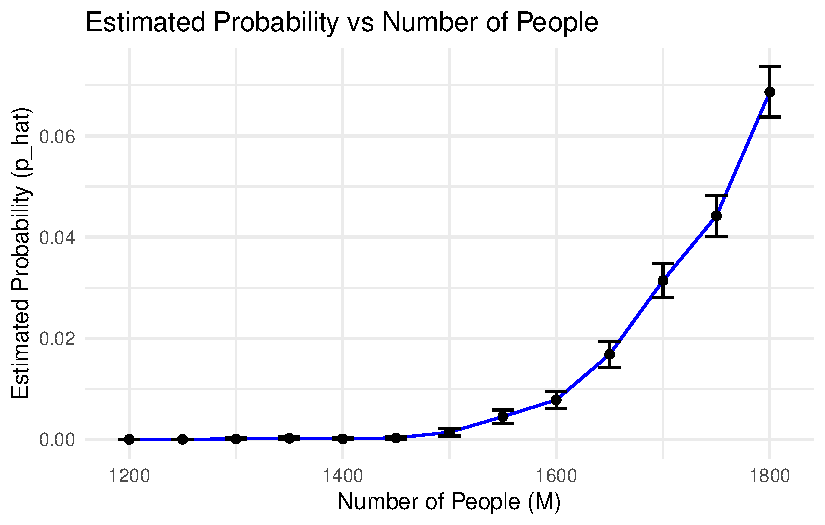
\includegraphics{Homework-4-BCA_files/figure-pdf/unnamed-chunk-6-1.pdf}

\subsubsection{\texorpdfstring{6. Finding \(M\) Such That
\(p_M = 0.5\)}{6. Finding M Such That p\_M = 0.5}}\label{finding-m-such-that-p_m-0.5}

We can interpolate to find \(M\) where \(\hat{p} \approx 0.5\):

\begin{Shaded}
\begin{Highlighting}[]
\NormalTok{approx\_M }\OtherTok{\textless{}{-}} \FunctionTok{approx}\NormalTok{(}\AttributeTok{x =}\NormalTok{ results}\SpecialCharTok{$}\NormalTok{p\_hat, }\AttributeTok{y =}\NormalTok{ results}\SpecialCharTok{$}\NormalTok{M, }\AttributeTok{xout =} \FloatTok{0.5}\NormalTok{)}\SpecialCharTok{$}\NormalTok{y}
\end{Highlighting}
\end{Shaded}

\begin{verbatim}
Warning in regularize.values(x, y, ties, missing(ties), na.rm = na.rm):
collapsing to unique 'x' values
\end{verbatim}

From the interpolation, we find:

\begin{itemize}
\tightlist
\item
  \(M \approx 1470\) gives \(\hat{p} \approx 0.5\).
\end{itemize}

\subsubsection{\texorpdfstring{7. Generalizing with Different \(B\)
Values}{7. Generalizing with Different B Values}}\label{generalizing-with-different-b-values}

We repeat the simulation for \(B = 10000, 50000, 100000\):

\begin{Shaded}
\begin{Highlighting}[]
\NormalTok{B\_values }\OtherTok{\textless{}{-}} \FunctionTok{c}\NormalTok{(}\DecValTok{10000}\NormalTok{, }\DecValTok{50000}\NormalTok{, }\DecValTok{100000}\NormalTok{)}
\NormalTok{all\_results }\OtherTok{\textless{}{-}} \FunctionTok{lapply}\NormalTok{(B\_values, }\ControlFlowTok{function}\NormalTok{(B) \{}
\NormalTok{  p\_estimates }\OtherTok{\textless{}{-}} \FunctionTok{sapply}\NormalTok{(M\_values, }\ControlFlowTok{function}\NormalTok{(M) }\FunctionTok{p\_hat}\NormalTok{(}\AttributeTok{M =}\NormalTok{ M, }\AttributeTok{B =}\NormalTok{ B))}
\NormalTok{  SE }\OtherTok{\textless{}{-}} \FunctionTok{sqrt}\NormalTok{(p\_estimates }\SpecialCharTok{*}\NormalTok{ (}\DecValTok{1} \SpecialCharTok{{-}}\NormalTok{ p\_estimates) }\SpecialCharTok{/}\NormalTok{ B)}
  \FunctionTok{data.frame}\NormalTok{(}\AttributeTok{M =}\NormalTok{ M\_values, }\AttributeTok{p\_hat =}\NormalTok{ p\_estimates, }\AttributeTok{SE =}\NormalTok{ SE, }\AttributeTok{B =}\NormalTok{ B)}
\NormalTok{\})}
\NormalTok{combined\_results }\OtherTok{\textless{}{-}} \FunctionTok{do.call}\NormalTok{(rbind, all\_results)}
\end{Highlighting}
\end{Shaded}

\subsubsection{\texorpdfstring{8. Comparing Results from Different \(B\)
Values}{8. Comparing Results from Different B Values}}\label{comparing-results-from-different-b-values}

We plot the results for each \(B\):

\begin{Shaded}
\begin{Highlighting}[]
\FunctionTok{ggplot}\NormalTok{(combined\_results, }\FunctionTok{aes}\NormalTok{(}\AttributeTok{x =}\NormalTok{ M, }\AttributeTok{y =}\NormalTok{ p\_hat, }\AttributeTok{color =} \FunctionTok{factor}\NormalTok{(B))) }\SpecialCharTok{+}
  \FunctionTok{geom\_line}\NormalTok{() }\SpecialCharTok{+}
  \FunctionTok{geom\_point}\NormalTok{() }\SpecialCharTok{+}
  \FunctionTok{labs}\NormalTok{(}\AttributeTok{title =} \StringTok{"Estimated Probability vs Number of People for Different B"}\NormalTok{,}
       \AttributeTok{x =} \StringTok{"Number of People (M)"}\NormalTok{,}
       \AttributeTok{y =} \StringTok{"Estimated Probability (p\_hat)"}\NormalTok{,}
       \AttributeTok{color =} \StringTok{"Number of Simulations (B)"}\NormalTok{) }\SpecialCharTok{+}
  \FunctionTok{theme\_minimal}\NormalTok{()}
\end{Highlighting}
\end{Shaded}

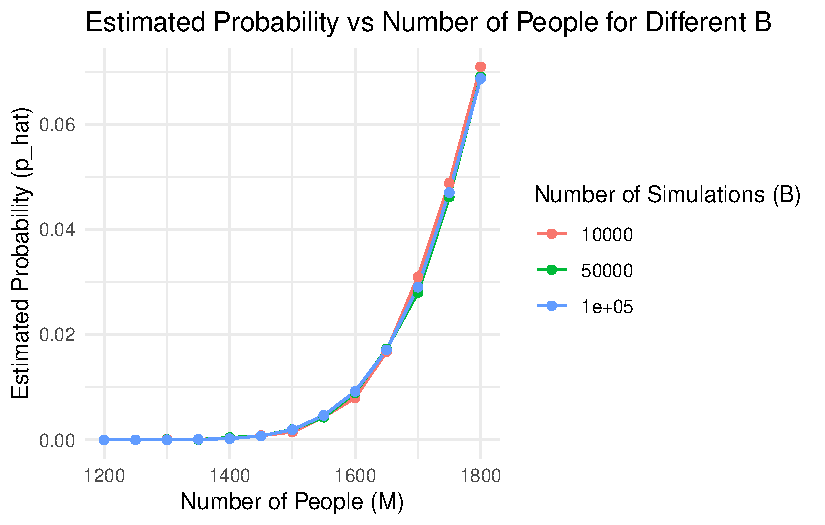
\includegraphics{Homework-4-BCA_files/figure-pdf/unnamed-chunk-9-1.pdf}

\textbf{Observations:}

\begin{itemize}
\tightlist
\item
  As \(B\) increases, the estimated probabilities become more precise
  (smaller \(SE\)).
\item
  The curves for different \(B\) values overlap, indicating consistency
  in the estimates.
\item
  The value of \(M\) where \(\hat{p} \approx 0.5\) remains around 1470
  across different \(B\).
\end{itemize}

\begin{center}\rule{0.5\linewidth}{0.5pt}\end{center}

\textbf{Conclusion:}

Through simulation, we estimate that approximately 1470 people are
needed for there to be a 50\% chance that every possible birthday is
represented. Increasing the number of simulations \(B\) improves the
accuracy of our estimates but does not significantly change the
estimated \(M\) value.




\end{document}
